% Options for packages loaded elsewhere
\PassOptionsToPackage{unicode}{hyperref}
\PassOptionsToPackage{hyphens}{url}
\documentclass[
]{article}
\usepackage{xcolor}
\usepackage{amsmath,amssymb}
\setcounter{secnumdepth}{-\maxdimen} % remove section numbering
\usepackage{iftex}
\ifPDFTeX
  \usepackage[T1]{fontenc}
  \usepackage[utf8]{inputenc}
  \usepackage{textcomp} % provide euro and other symbols
\else % if luatex or xetex
  \usepackage{unicode-math} % this also loads fontspec
  \defaultfontfeatures{Scale=MatchLowercase}
  \defaultfontfeatures[\rmfamily]{Ligatures=TeX,Scale=1}
\fi
\usepackage{lmodern}
\ifPDFTeX\else
  % xetex/luatex font selection
\fi
% Use upquote if available, for straight quotes in verbatim environments
\IfFileExists{upquote.sty}{\usepackage{upquote}}{}
\IfFileExists{microtype.sty}{% use microtype if available
  \usepackage[]{microtype}
  \UseMicrotypeSet[protrusion]{basicmath} % disable protrusion for tt fonts
}{}
\makeatletter
\@ifundefined{KOMAClassName}{% if non-KOMA class
  \IfFileExists{parskip.sty}{%
    \usepackage{parskip}
  }{% else
    \setlength{\parindent}{0pt}
    \setlength{\parskip}{6pt plus 2pt minus 1pt}}
}{% if KOMA class
  \KOMAoptions{parskip=half}}
\makeatother
\usepackage{color}
\usepackage{fancyvrb}
\newcommand{\VerbBar}{|}
\newcommand{\VERB}{\Verb[commandchars=\\\{\}]}
\DefineVerbatimEnvironment{Highlighting}{Verbatim}{commandchars=\\\{\}}
% Add ',fontsize=\small' for more characters per line
\newenvironment{Shaded}{}{}
\newcommand{\AlertTok}[1]{\textcolor[rgb]{1.00,0.00,0.00}{\textbf{#1}}}
\newcommand{\AnnotationTok}[1]{\textcolor[rgb]{0.38,0.63,0.69}{\textbf{\textit{#1}}}}
\newcommand{\AttributeTok}[1]{\textcolor[rgb]{0.49,0.56,0.16}{#1}}
\newcommand{\BaseNTok}[1]{\textcolor[rgb]{0.25,0.63,0.44}{#1}}
\newcommand{\BuiltInTok}[1]{\textcolor[rgb]{0.00,0.50,0.00}{#1}}
\newcommand{\CharTok}[1]{\textcolor[rgb]{0.25,0.44,0.63}{#1}}
\newcommand{\CommentTok}[1]{\textcolor[rgb]{0.38,0.63,0.69}{\textit{#1}}}
\newcommand{\CommentVarTok}[1]{\textcolor[rgb]{0.38,0.63,0.69}{\textbf{\textit{#1}}}}
\newcommand{\ConstantTok}[1]{\textcolor[rgb]{0.53,0.00,0.00}{#1}}
\newcommand{\ControlFlowTok}[1]{\textcolor[rgb]{0.00,0.44,0.13}{\textbf{#1}}}
\newcommand{\DataTypeTok}[1]{\textcolor[rgb]{0.56,0.13,0.00}{#1}}
\newcommand{\DecValTok}[1]{\textcolor[rgb]{0.25,0.63,0.44}{#1}}
\newcommand{\DocumentationTok}[1]{\textcolor[rgb]{0.73,0.13,0.13}{\textit{#1}}}
\newcommand{\ErrorTok}[1]{\textcolor[rgb]{1.00,0.00,0.00}{\textbf{#1}}}
\newcommand{\ExtensionTok}[1]{#1}
\newcommand{\FloatTok}[1]{\textcolor[rgb]{0.25,0.63,0.44}{#1}}
\newcommand{\FunctionTok}[1]{\textcolor[rgb]{0.02,0.16,0.49}{#1}}
\newcommand{\ImportTok}[1]{\textcolor[rgb]{0.00,0.50,0.00}{\textbf{#1}}}
\newcommand{\InformationTok}[1]{\textcolor[rgb]{0.38,0.63,0.69}{\textbf{\textit{#1}}}}
\newcommand{\KeywordTok}[1]{\textcolor[rgb]{0.00,0.44,0.13}{\textbf{#1}}}
\newcommand{\NormalTok}[1]{#1}
\newcommand{\OperatorTok}[1]{\textcolor[rgb]{0.40,0.40,0.40}{#1}}
\newcommand{\OtherTok}[1]{\textcolor[rgb]{0.00,0.44,0.13}{#1}}
\newcommand{\PreprocessorTok}[1]{\textcolor[rgb]{0.74,0.48,0.00}{#1}}
\newcommand{\RegionMarkerTok}[1]{#1}
\newcommand{\SpecialCharTok}[1]{\textcolor[rgb]{0.25,0.44,0.63}{#1}}
\newcommand{\SpecialStringTok}[1]{\textcolor[rgb]{0.73,0.40,0.53}{#1}}
\newcommand{\StringTok}[1]{\textcolor[rgb]{0.25,0.44,0.63}{#1}}
\newcommand{\VariableTok}[1]{\textcolor[rgb]{0.10,0.09,0.49}{#1}}
\newcommand{\VerbatimStringTok}[1]{\textcolor[rgb]{0.25,0.44,0.63}{#1}}
\newcommand{\WarningTok}[1]{\textcolor[rgb]{0.38,0.63,0.69}{\textbf{\textit{#1}}}}
\usepackage{graphicx}
\makeatletter
\newsavebox\pandoc@box
\newcommand*\pandocbounded[1]{% scales image to fit in text height/width
  \sbox\pandoc@box{#1}%
  \Gscale@div\@tempa{\textheight}{\dimexpr\ht\pandoc@box+\dp\pandoc@box\relax}%
  \Gscale@div\@tempb{\linewidth}{\wd\pandoc@box}%
  \ifdim\@tempb\p@<\@tempa\p@\let\@tempa\@tempb\fi% select the smaller of both
  \ifdim\@tempa\p@<\p@\scalebox{\@tempa}{\usebox\pandoc@box}%
  \else\usebox{\pandoc@box}%
  \fi%
}
% Set default figure placement to htbp
\def\fps@figure{htbp}
\makeatother
\usepackage{svg}
\ifLuaTeX
\usepackage[bidi=basic]{babel}
\else
\usepackage[bidi=default]{babel}
\fi
\babelprovide[main,import]{french}
% get rid of language-specific shorthands (see #6817):
\let\LanguageShortHands\languageshorthands
\def\languageshorthands#1{}
\setlength{\emergencystretch}{3em} % prevent overfull lines
\providecommand{\tightlist}{%
  \setlength{\itemsep}{0pt}\setlength{\parskip}{0pt}}
\usepackage{bookmark}
\IfFileExists{xurl.sty}{\usepackage{xurl}}{} % add URL line breaks if available
\urlstyle{same}
\hypersetup{
  pdftitle={3~ Réhaussement et visualisation d'images -- Traitement d\textquotesingle images satellites avec Python},
  pdflang={fr},
  hidelinks,
  pdfcreator={LaTeX via pandoc}}

\title{3~ Réhaussement et visualisation d'images -- Traitement
d\textquotesingle images satellites avec Python}
\author{}
\date{}

\begin{document}
\maketitle

\phantomsection\label{quarto-document-content}
\phantomsection\label{title-block-header}
\section{\texorpdfstring{\protect\hypertarget{sec-chap02}{}{{3}~
{Réhaussement et visualisation
d'images}}}{3~ Réhaussement et visualisation d'images}}\label{ruxe9haussement-et-visualisation-dimages}

Assurez-vous de lire ce préambule avant d'exécutez le reste du notebook.

\subsection{\texorpdfstring{{3.1} {🚀}
Préambule}{3.1 🚀 Préambule}}\label{pruxe9ambule}

\subsubsection{\texorpdfstring{{3.1.1} {🎯}
Objectifs}{3.1.1 🎯 Objectifs}}\label{objectifs}

Dans ce chapitre, nous abordons quelques techniques de réhaussement et
de visualisation d'images. Ce chapitre est aussi disponible sous la
forme d'un notebook Python:

\href{https://colab.research.google.com/github/sfoucher/TraitementImagesPythonVol1/blob/main/notebooks/02-RehaussementVisualisationImages.ipynb}{\pandocbounded{\includesvg[keepaspectratio]{images/colab-badge.svg}}}

\subsubsection{\texorpdfstring{{3.1.2}
Librairies}{3.1.2 Librairies}}\label{librairies}

Les librairies qui vont être explorées dans ce chapitre sont les
suivantes:

\begin{itemize}
\item
  \href{https://scipy.org/}{SciPy -}
\item
  \href{https://numpy.org/}{NumPy -}
\item
  \href{https://pypi.org/project/opencv-python/}{opencv-python · PyPI}
\item
  \href{https://scikit-image.org/}{scikit-image}
\item
  \href{https://rasterio.readthedocs.io/en/stable/}{Rasterio}
\item
  \href{https://docs.xarray.dev/en/stable/}{Xarray}
\item
  \href{https://corteva.github.io/rioxarray/stable/index.html}{rioxarray}
\end{itemize}

Dans l'environnement Google Colab, seul \texttt{rioxarray} et GDAL
doivent être installés:

\phantomsection\label{5eee1e9a}
\phantomsection\label{cb1}
\begin{Shaded}
\begin{Highlighting}[]
\OperatorTok{\%\%}\NormalTok{capture}
\OperatorTok{!}\NormalTok{apt}\OperatorTok{{-}}\NormalTok{get update}
\OperatorTok{!}\NormalTok{apt}\OperatorTok{{-}}\NormalTok{get install gdal}\OperatorTok{{-}}\BuiltInTok{bin}\NormalTok{ libgdal}\OperatorTok{{-}}\NormalTok{dev}
\OperatorTok{!}\NormalTok{pip install }\OperatorTok{{-}}\NormalTok{q rioxarray}
\OperatorTok{!}\NormalTok{pip install }\OperatorTok{{-}}\NormalTok{qU }\StringTok{"geemap[workshop]"}
\end{Highlighting}
\end{Shaded}

Vérifier les importations:

\phantomsection\label{1382991a}
\phantomsection\label{cb2}
\begin{Shaded}
\begin{Highlighting}[]
\ImportTok{import}\NormalTok{ numpy }\ImportTok{as}\NormalTok{ np}
\ImportTok{import}\NormalTok{ rioxarray }\ImportTok{as}\NormalTok{ rxr}
\ImportTok{from}\NormalTok{ scipy }\ImportTok{import}\NormalTok{ signal}
\ImportTok{import}\NormalTok{ xarray }\ImportTok{as}\NormalTok{ xr}
\ImportTok{import}\NormalTok{ xrscipy}
\ImportTok{import}\NormalTok{ matplotlib.pyplot }\ImportTok{as}\NormalTok{ plt}
\end{Highlighting}
\end{Shaded}

\subsubsection{\texorpdfstring{{3.1.3}
Données}{3.1.3 Données}}\label{donnuxe9es}

Nous allons utilisez les images suivantes dans ce chapitre:

\phantomsection\label{bb158c30}
\phantomsection\label{cb3}
\begin{Shaded}
\begin{Highlighting}[]
\OperatorTok{\%\%}\NormalTok{capture}
\OperatorTok{!}\NormalTok{wget https:}\OperatorTok{//}\NormalTok{github.com}\OperatorTok{/}\NormalTok{sfoucher}\OperatorTok{/}\NormalTok{TraitementImagesPythonVol1}\OperatorTok{/}\NormalTok{raw}\OperatorTok{/}\NormalTok{refs}\OperatorTok{/}\NormalTok{heads}\OperatorTok{/}\NormalTok{main}\OperatorTok{/}\NormalTok{data}\OperatorTok{/}\NormalTok{chapitre01}\OperatorTok{/}\NormalTok{subset\_RGBNIR\_of\_S2A\_MSIL2A\_20240625T153941\_N0510\_R011\_T18TYR\_20240625T221903.tif }\OperatorTok{{-}}\NormalTok{O RGBNIR\_of\_S2A.tif}
\OperatorTok{!}\NormalTok{wget https:}\OperatorTok{//}\NormalTok{github.com}\OperatorTok{/}\NormalTok{sfoucher}\OperatorTok{/}\NormalTok{opengeos}\OperatorTok{{-}}\NormalTok{data}\OperatorTok{/}\NormalTok{raw}\OperatorTok{/}\NormalTok{refs}\OperatorTok{/}\NormalTok{heads}\OperatorTok{/}\NormalTok{main}\OperatorTok{/}\NormalTok{raster}\OperatorTok{/}\NormalTok{landsat7.tif }\OperatorTok{{-}}\NormalTok{O landsat7.tif}
\OperatorTok{!}\NormalTok{wget https:}\OperatorTok{//}\NormalTok{github.com}\OperatorTok{/}\NormalTok{sfoucher}\OperatorTok{/}\NormalTok{opengeos}\OperatorTok{{-}}\NormalTok{data}\OperatorTok{/}\NormalTok{raw}\OperatorTok{/}\NormalTok{refs}\OperatorTok{/}\NormalTok{heads}\OperatorTok{/}\NormalTok{main}\OperatorTok{/}\NormalTok{images}\OperatorTok{/}\NormalTok{berkeley.jpg }\OperatorTok{{-}}\NormalTok{O berkeley.jpg}
\OperatorTok{!}\NormalTok{wget https:}\OperatorTok{//}\NormalTok{github.com}\OperatorTok{/}\NormalTok{sfoucher}\OperatorTok{/}\NormalTok{TraitementImagesPythonVol1}\OperatorTok{/}\NormalTok{raw}\OperatorTok{/}\NormalTok{refs}\OperatorTok{/}\NormalTok{heads}\OperatorTok{/}\NormalTok{main}\OperatorTok{/}\NormalTok{data}\OperatorTok{/}\NormalTok{chapitre01}\OperatorTok{/}\NormalTok{subset\_0\_of\_S1A\_split\_NR\_Cal\_Deb\_ML\_Spk\_SRGR.tif }\OperatorTok{{-}}\NormalTok{O SAR.tif}
\end{Highlighting}
\end{Shaded}

Vérifiez que vous êtes capable de les lire :

\phantomsection\label{3d6a2976}
\phantomsection\label{cb4}
\begin{Shaded}
\begin{Highlighting}[]
\ControlFlowTok{with}\NormalTok{ rxr.open\_rasterio(}\StringTok{\textquotesingle{}berkeley.jpg\textquotesingle{}}\NormalTok{, mask\_and\_scale}\OperatorTok{=} \VariableTok{True}\NormalTok{) }\ImportTok{as}\NormalTok{ img\_rgb:}
    \BuiltInTok{print}\NormalTok{(img\_rgb)}
\ControlFlowTok{with}\NormalTok{ rxr.open\_rasterio(}\StringTok{\textquotesingle{}RGBNIR\_of\_S2A.tif\textquotesingle{}}\NormalTok{, mask\_and\_scale}\OperatorTok{=} \VariableTok{True}\NormalTok{) }\ImportTok{as}\NormalTok{ img\_rgbnir:}
    \BuiltInTok{print}\NormalTok{(img\_rgbnir)}
\ControlFlowTok{with}\NormalTok{ rxr.open\_rasterio(}\StringTok{\textquotesingle{}SAR.tif\textquotesingle{}}\NormalTok{, mask\_and\_scale}\OperatorTok{=} \VariableTok{True}\NormalTok{) }\ImportTok{as}\NormalTok{ img\_SAR:}
    \BuiltInTok{print}\NormalTok{(img\_SAR)}
\end{Highlighting}
\end{Shaded}

\subsection{\texorpdfstring{{3.2} Réhaussements
visuels}{3.2 Réhaussements visuels}}\label{ruxe9haussements-visuels}

Le but du réhaussement visuel d'une image vise principalement à
améliorer la qualité visuelle d'une image en améliorant le contraste, la
dynamique ou la texture d'une image. De manière générale, ce
réhaussement ne modifie pas la donnée d'origine mais est plutôt
appliquée dynamiquement à l'affichage pour des fins d'inspection
visuelle.

\subsubsection{\texorpdfstring{{3.2.1} Statistiques d'une
image}{3.2.1 Statistiques d'une image}}\label{statistiques-dune-image}

On peut considérer un ensemble de statistique globales pour chacune des
bandes d'une image: - valeurs minimales et maximales - valeurs moyennes,
médianes et quantiles - écart-types, skewness et kurtosis Ces
statistiques doivent être calculées pour chaque bande d'une image
multispectrale.

En ligne de commande, \texttt{gdalinfo} permet d'interroger rapidement
un fichier image pour connaitre les statistiques de base:

\phantomsection\label{a2a1248d}
\phantomsection\label{lst-gdalstats}
\begin{figure}
\centering
\phantomsection\label{lst-gdalstats}
\begin{Shaded}
\begin{Highlighting}[]
\OperatorTok{!}\NormalTok{gdalinfo }\OperatorTok{{-}}\NormalTok{stats landsat7.tif}
\end{Highlighting}
\end{Shaded}
\caption{Bloc de code~3.1: Statistiques d'une image avec gdal}
\end{figure}

\begin{verbatim}
Driver: GTiff/GeoTIFF
Files: landsat7.tif
       landsat7.tif.aux.xml
Size is 2181, 1917
Coordinate System is:
PROJCS["WGS 84 / Pseudo-Mercator",
    GEOGCS["WGS 84",
        DATUM["WGS_1984",
            SPHEROID["WGS 84",6378137,298.257223563,
                AUTHORITY["EPSG","7030"]],
            AUTHORITY["EPSG","6326"]],
        PRIMEM["Greenwich",0,
            AUTHORITY["EPSG","8901"]],
        UNIT["degree",0.0174532925199433,
            AUTHORITY["EPSG","9122"]],
        AUTHORITY["EPSG","4326"]],
    PROJECTION["Mercator_1SP"],
    PARAMETER["central_meridian",0],
    PARAMETER["scale_factor",1],
    PARAMETER["false_easting",0],
    PARAMETER["false_northing",0],
    UNIT["metre",1,
        AUTHORITY["EPSG","9001"]],
    AXIS["X",EAST],
    AXIS["Y",NORTH],
    EXTENSION["PROJ4","+proj=merc +a=6378137 +b=6378137 +lat_ts=0.0 +lon_0=0.0 +x_0=0.0 +y_0=0 +k=1.0 +units=m +nadgrids=@null +wktext +no_defs"],
    AUTHORITY["EPSG","3857"]]
Origin = (-13651650.000000000000000,4576290.000000000000000)
Pixel Size = (30.000000000000000,-30.000000000000000)
Metadata:
  AREA_OR_POINT=Area
  OVR_RESAMPLING_ALG=NEAREST
  TIFFTAG_RESOLUTIONUNIT=1 (unitless)
  TIFFTAG_XRESOLUTION=1
  TIFFTAG_YRESOLUTION=1
Image Structure Metadata:
  COMPRESSION=DEFLATE
  INTERLEAVE=PIXEL
Corner Coordinates:
Upper Left  (-13651650.000, 4576290.000) (122d38' 5.49"W, 37d58'40.08"N)
Lower Left  (-13651650.000, 4518780.000) (122d38' 5.49"W, 37d34'10.00"N)
Upper Right (-13586220.000, 4576290.000) (122d 2'49.53"W, 37d58'40.08"N)
Lower Right (-13586220.000, 4518780.000) (122d 2'49.53"W, 37d34'10.00"N)
Center      (-13618935.000, 4547535.000) (122d20'27.51"W, 37d46'26.05"N)
Band 1 Block=512x512 Type=Byte, ColorInterp=Red
  Min=19.000 Max=233.000 
  Minimum=19.000, Maximum=233.000, Mean=98.433, StdDev=21.164
  NoData Value=0
  Overviews: 1091x959, 546x480
  Metadata:
    STATISTICS_MAXIMUM=233
    STATISTICS_MEAN=98.433096940153
    STATISTICS_MINIMUM=19
    STATISTICS_STDDEV=21.164021026458
Band 2 Block=512x512 Type=Byte, ColorInterp=Green
  Min=19.000 Max=178.000 
  Minimum=19.000, Maximum=178.000, Mean=55.068, StdDev=22.204
  NoData Value=0
  Overviews: 1091x959, 546x480
  Metadata:
    STATISTICS_MAXIMUM=178
    STATISTICS_MEAN=55.067787534804
    STATISTICS_MINIMUM=19
    STATISTICS_STDDEV=22.203571974581
Band 3 Block=512x512 Type=Byte, ColorInterp=Blue
  Min=19.000 Max=187.000 
  Minimum=19.000, Maximum=187.000, Mean=43.341, StdDev=20.330
  NoData Value=0
  Overviews: 1091x959, 546x480
  Metadata:
    STATISTICS_MAXIMUM=187
    STATISTICS_MEAN=43.340507443056
    STATISTICS_MINIMUM=19
    STATISTICS_STDDEV=20.32987736339
\end{verbatim}

Les librairies de base comme \texttt{xarray} et \texttt{numpy} peuvent
facilement produire des statistiques comme avec la fonction
\href{https://rasterio.readthedocs.io/en/stable/api/rasterio.io.html\#rasterio.io.BufferedDatasetWriter.stats}{stats}:

\phantomsection\label{093601ed}
\phantomsection\label{cb6}
\begin{Shaded}
\begin{Highlighting}[]
\ImportTok{import}\NormalTok{ rasterio }\ImportTok{as}\NormalTok{ rio}
\ImportTok{import}\NormalTok{ numpy }\ImportTok{as}\NormalTok{ np}
\ControlFlowTok{with}\NormalTok{ rio.}\BuiltInTok{open}\NormalTok{(}\StringTok{\textquotesingle{}landsat7.tif\textquotesingle{}}\NormalTok{) }\ImportTok{as}\NormalTok{ src:}
\NormalTok{    stats}\OperatorTok{=}\NormalTok{ src.stats()}
    \BuiltInTok{print}\NormalTok{(stats)}
\end{Highlighting}
\end{Shaded}

La librairie \texttt{xarray} donne accès à des fonctionnalités plus
sophistiquées comme le calcul des quantiles:

\phantomsection\label{28aa5d49}
\phantomsection\label{cb7}
\begin{Shaded}
\begin{Highlighting}[]
\ImportTok{import}\NormalTok{ rioxarray }\ImportTok{as}\NormalTok{ riox}
\ControlFlowTok{with}\NormalTok{ riox.open\_rasterio(}\StringTok{\textquotesingle{}landsat7.tif\textquotesingle{}}\NormalTok{, masked}\OperatorTok{=} \VariableTok{True}\NormalTok{) }\ImportTok{as}\NormalTok{ src:}
    \BuiltInTok{print}\NormalTok{(src)}
\NormalTok{quantiles }\OperatorTok{=}\NormalTok{ src.quantile(dim}\OperatorTok{=}\NormalTok{[}\StringTok{\textquotesingle{}x\textquotesingle{}}\NormalTok{,}\StringTok{\textquotesingle{}y\textquotesingle{}}\NormalTok{], q}\OperatorTok{=}\NormalTok{[}\FloatTok{.025}\NormalTok{,}\FloatTok{.25}\NormalTok{,}\FloatTok{.5}\NormalTok{,}\FloatTok{.75}\NormalTok{,}\FloatTok{.975}\NormalTok{])}
\NormalTok{quantiles}
\end{Highlighting}
\end{Shaded}

\begin{verbatim}
<xarray.DataArray (band: 3, y: 1917, x: 2181)> Size: 50MB
[12542931 values with dtype=float32]
Coordinates:
  * band         (band) int64 24B 1 2 3
  * x            (x) float64 17kB -1.365e+07 -1.365e+07 ... -1.359e+07
  * y            (y) float64 15kB 4.576e+06 4.576e+06 ... 4.519e+06 4.519e+06
    spatial_ref  int64 8B 0
Attributes:
    AREA_OR_POINT:           Area
    OVR_RESAMPLING_ALG:      NEAREST
    TIFFTAG_RESOLUTIONUNIT:  1 (unitless)
    TIFFTAG_XRESOLUTION:     1
    TIFFTAG_YRESOLUTION:     1
    STATISTICS_MAXIMUM:      233
    STATISTICS_MEAN:         98.433096940153
    STATISTICS_MINIMUM:      19
    STATISTICS_STDDEV:       21.164021026458
    scale_factor:            1.0
    add_offset:              0.0
\end{verbatim}

\begin{Shaded}
\begin{Highlighting}[]
\NormalTok{\textless{}xarray.DataArray (quantile: 5, band: 3)\textgreater{} Size: 120B}
\NormalTok{array([[ 54.,  19.,  19.],}
\NormalTok{       [ 85.,  38.,  27.],}
\NormalTok{       [ 99.,  54.,  38.],}
\NormalTok{       [111.,  69.,  57.],}
\NormalTok{       [140., 102.,  89.]])}
\NormalTok{Coordinates:}
\NormalTok{  * band      (band) int64 24B 1 2 3}
\NormalTok{  * quantile  (quantile) float64 40B 0.025 0.25 0.5 0.75 0.975}
\end{Highlighting}
\end{Shaded}

xarray.DataArray

\begin{itemize}
\tightlist
\item
  {quantile}: 5
\item
  {band}: 3
\end{itemize}

{54.0 19.0 19.0 85.0 38.0 27.0 ... 111.0 69.0 57.0 140.0 102.0 89.0}

\begin{verbatim}
array([[ 54.,  19.,  19.],
       [ 85.,  38.,  27.],
       [ 99.,  54.,  38.],
       [111.,  69.,  57.],
       [140., 102.,  89.]])
\end{verbatim}

Coordinates: {(2)}

{band}

(band)

int64

1 2 3

\begin{verbatim}
array([1, 2, 3])
\end{verbatim}

{quantile}

(quantile)

float64

0.025 0.25 0.5 0.75 0.975

\begin{verbatim}
array([0.025, 0.25 , 0.5  , 0.75 , 0.975])
\end{verbatim}

Indexes: {(2)}

band

PandasIndex

\begin{verbatim}
PandasIndex(Index([1, 2, 3], dtype='int64', name='band'))
\end{verbatim}

quantile

PandasIndex

\begin{verbatim}
PandasIndex(Index([0.025, 0.25, 0.5, 0.75, 0.975], dtype='float64', name='quantile'))
\end{verbatim}

Attributes: {(0)}

\paragraph{\texorpdfstring{{3.2.1.1} Calcul de
l'histogramme}{3.2.1.1 Calcul de l'histogramme}}\label{calcul-de-lhistogramme}

Le calcul d'un histogramme pour une image (une bande) permet d'avoir une
vue plus détaillée de la répartition des valeurs radiométriques. Le
calcul d'un histogramme nécessite minimalement de faire le choix d'une
valeur du nombre de \emph{bins} (ou de la largeur). Un \emph{bin} est un
intervalle de valeurs pour lequel on peut calculer le nombre de valeurs
observées dans l'image. La fonction de base pour ce type de calcul est
la fonction \texttt{numpy.histogram()}:

\phantomsection\label{970fff3f}
\phantomsection\label{cb9}
\begin{Shaded}
\begin{Highlighting}[]
\ImportTok{import}\NormalTok{ numpy }\ImportTok{as}\NormalTok{ np}
\NormalTok{array }\OperatorTok{=}\NormalTok{ np.random.randint(}\DecValTok{0}\NormalTok{,}\DecValTok{10}\NormalTok{,}\DecValTok{100}\NormalTok{) }\CommentTok{\# 100 valeurs aléatoires entre 0 et 10}
\NormalTok{hist, bin\_limites }\OperatorTok{=}\NormalTok{ np.histogram(array, density}\OperatorTok{=}\VariableTok{True}\NormalTok{)}
\BuiltInTok{print}\NormalTok{(}\StringTok{\textquotesingle{}valeurs :\textquotesingle{}}\NormalTok{,hist)}
\BuiltInTok{print}\NormalTok{(}\StringTok{\textquotesingle{};imites :\textquotesingle{}}\NormalTok{,bin\_limites)}
\end{Highlighting}
\end{Shaded}

\begin{verbatim}
valeurs : [0.11111111 0.16666667 0.12222222 0.06666667 0.07777778 0.11111111
 0.11111111 0.08888889 0.16666667 0.08888889]
;imites : [0.  0.9 1.8 2.7 3.6 4.5 5.4 6.3 7.2 8.1 9. ]
\end{verbatim}

Le calcul se fait avec 10 intervalles par défaut.

Pour des besoins de visualisation, le calcul des valeurs extrêmes de
l'histogramme peut aussi se faire via les quantiles comme discutés
auparavant.

\subparagraph{\texorpdfstring{{3.2.1.1.1} Visualisation des
histogrammes}{3.2.1.1.1 Visualisation des histogrammes}}\label{visualisation-des-histogrammes}

La librarie \texttt{rasterio} est probablement l'outil le plus simples
pour visualiser rapidement des histogrammes sur une image
multi-spectrale:

\phantomsection\label{a0c4ddee}
\phantomsection\label{cb11}
\begin{Shaded}
\begin{Highlighting}[]
\ImportTok{import}\NormalTok{ rasterio }\ImportTok{as}\NormalTok{ rio}
\ImportTok{from}\NormalTok{ rasterio.plot }\ImportTok{import}\NormalTok{ show\_hist}
\ControlFlowTok{with}\NormalTok{ rio.}\BuiltInTok{open}\NormalTok{(}\StringTok{\textquotesingle{}RGBNIR\_of\_S2A.tif\textquotesingle{}}\NormalTok{) }\ImportTok{as}\NormalTok{ src:}
\NormalTok{  show\_hist(src, bins}\OperatorTok{=}\DecValTok{50}\NormalTok{, lw}\OperatorTok{=}\FloatTok{0.0}\NormalTok{, stacked}\OperatorTok{=}\VariableTok{False}\NormalTok{, alpha}\OperatorTok{=}\FloatTok{0.3}\NormalTok{,histtype}\OperatorTok{=}\StringTok{\textquotesingle{}stepfilled\textquotesingle{}}\NormalTok{, title}\OperatorTok{=}\StringTok{"Histogram"}\NormalTok{)}
\end{Highlighting}
\end{Shaded}

\begin{figure}
\centering
\pandocbounded{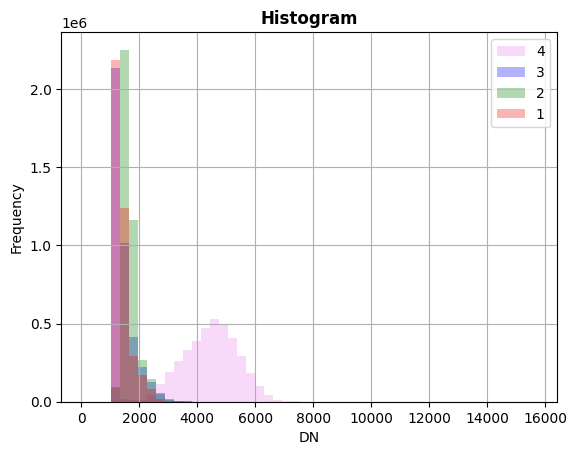
\includegraphics[keepaspectratio]{02-RehaussementVisualisationImages_files/figure-html/cell-10-output-1.png}}
\caption{}
\end{figure}

\subsubsection{\texorpdfstring{{3.2.2} Réhaussements
linéaires}{3.2.2 Réhaussements linéaires}}\label{ruxe9haussements-linuxe9aires}

Le réhaussement linéaire d'une image est la forme la plus simple de
réhaussement, elle consiste 1) à optimiser les valeurs des pixels d'une
image afin de maximiser la dynamique disponibles à l'affichage, ou 2)
changer le format de stockage des valeurs (e.g.~de 8 bit à 16 bit):

\phantomsection\label{eq-rehauss-lin}{{\textbackslash{[}
\textbackslash text\{nouvelle valeur d\textquotesingle un pixel\} =
\textbackslash frac\{\textbackslash text\{valeur d\textquotesingle un
pixel\} - min\_0\}\{max\_0 - min\_0\}\textbackslash times (max\_1 -
min\_1)+min\_1 \textbackslash tag\{3.1\}\textbackslash{]}}}

Par cette opération, on passe de la dynamique de départ
({\textbackslash(max\_0 - min\_0\textbackslash)}) vers la dynamique
cible ({\textbackslash(max\_1 - min\_1\textbackslash)}). Bien que cette
opération semble triviale, il est important d'être conscient des trois
contraintes suivantes: 1. \textbf{Faire attention à la dynamique cible},
ainsi, pour sauvegarder une image en format 8 bit, on utilisera alors
{\textbackslash(max\_1=255\textbackslash)} et
{\textbackslash(min\_1=0\textbackslash)}. 2. \textbf{Préservation de la
valeur de no data} : il faut faire attention à la valeur
{\textbackslash(min\_1\textbackslash)} dans le cas d'une valeur présente
pour \emph{no\_data}. Par exemple, si \emph{no\_data=0} alors il faut
s'assurer que {\textbackslash(min\_1\textgreater0\textbackslash)}. 3.
\textbf{Précision du calcul} : si possible réaliser la division
ci-dessus en format \emph{float}

\subsubsection{\texorpdfstring{{3.2.3} Réhaussements non
linéaires}{3.2.3 Réhaussements non linéaires}}\label{ruxe9haussements-non-linuxe9aires}

Calcul d'histogrammes, étirement, égalisation, styling

\subsubsection{\texorpdfstring{{3.2.4} Composés
couleurs}{3.2.4 Composés couleurs}}\label{composuxe9s-couleurs}

Le système visuel humain est sensible seulement à la partie visible du
spectre électromagnétique qui compose les couleurs de l'arc-en-ciel du
bleu au rouge. L'ensemble des couleurs du spectre visible peut être
obtenu à partir du mélange de trois couleurs primaires (rouge, vert et
bleu). Ce système de décomposition à trois couleurs est à la base de la
plupart des systèmes de visualisation ou de représentation de
l'information de couleur. On peut trouver des variantes comme le système
HSV (\emph{Hue-Saturation-Value}) utilisé en encodage de données vidéos.

\subsection{\texorpdfstring{{3.3}
Visualisation}{3.3 Visualisation}}\label{visualisation}

\subsubsection{\texorpdfstring{{3.3.1} Visualisation en
Python}{3.3.1 Visualisation en Python}}\label{visualisation-en-python}

Il faut d'entrée mentionner que Python n'est pas vraiment fait pour
visualiser de la donnée de grande taille, le niveau d'interactivité est
aussi plus limité. Néanmoins, il est possible de visualiser de petites
images avec la librairie Matplotlib.

\subsubsection{\texorpdfstring{{3.3.2} Outils de
visualisation}{3.3.2 Outils de visualisation}}\label{outils-de-visualisation}

Il existe plusieurs outils gratuits de visualisation d'une image
satellite, on peut mentionner les deux principaux: - QGIS - ESA Snap

\subsubsection{\texorpdfstring{{3.3.3} Visualisation sur le
Web}{3.3.3 Visualisation sur le Web}}\label{visualisation-sur-le-web}

Une des meilleures pratiques pour visualiser une image de grande taille
est d'utiliser un service de type Web Mapping Service (WMS). Cependant,
type de service nécessite une architecture client-serveur qui est plus
complexe à mettre en place.

Google Earth Engine offre des moyens de visualiser de la donnée locale:
\emph{Working with Local Geospatial Data} --- via
\href{https://geog-312.gishub.org/book/geospatial/geemap.html\#working-with-local-geospatial-data}{17.
Geemap --- Introduction to GIS Programming}

via \href{https://github.com/opengeos/data/tree/main/raster}{data/raster
at main · opengeos/data}

\subsubsection{\texorpdfstring{{3.3.4} Visualisation
3D}{3.3.4 Visualisation 3D}}\label{visualisation-3d}

drapper une image satellite sur un DEM

\subsection{\texorpdfstring{{3.4} Exercices de
révision}{3.4 Exercices de révision}}\label{exercices-de-ruxe9vision}

\end{document}
